\documentclass{article}
\usepackage[utf8]{inputenc}
\usepackage{pgfplots}
\pgfplotsset{width=6.6cm,compat=1.7}
\usepackage{parskip}

\usepackage[backend=bibtex]{biblatex}
\addbibresource{sources.bib}

% has to be the last package to import
\usepackage{hyperref}
\hypersetup{
    colorlinks=true,
    citecolor=blue,
    linkcolor=black,
    filecolor=magenta,
    urlcolor=blue,
}
\urlstyle{same}

% Extra vertical spacing for each paragraph
\setlength\parindent{16pt}


\title{Unity game performance difference between Vulkan and WebGL in Linux}
\author{Erik Reider}
\date{\today}

\begin{document}

% Title
\maketitle
\newpage

% Abstract
\begin{abstract}
In this thesis, I compared the CPU performance differences between Vulkan and WebGL2 in Chromium and Firefox on Linux. The benchmarks were made in the Unity 3D game engine using C\#. All tests were run on a high-end and a low-end PC and graphed accordingly (figure[\ref{fig:test1}] and figure[\ref{fig:test2}]). The benchmarks tested two CPU heavy loads, raw CPU performance and draw call performance. While testing, OpenGL was used as a control to more easily verify the results because of WebGL being a more lightweight version of OpenGL. The Vulkan results were significantly faster than the WebGL results because of significant overhead created by the browser while the OpenGL results were comparable to the Vulkan results. The conclusion concluded that compiling to a PC natively is the best option when every last drop of performance matters but not when wanting the best cross-compatibility support where the web version shines the most.
\end{abstract}

\newpage


% Tabel of content
\tableofcontents
\listoffigures
\newpage


\section {Introduction}
When creating a game, a programmer can choose where their game will be played. Depending on the platform, it could either be really simple or extremely difficult. The Unity game engine (also referred to as Unity) is a game creation tool that is considered to be one of the best game engines in the world. Unity can build games for Windows, Linux, Mac OS, Android, iOS, every modern console and your web browser. Should one consider publishing ones game to all platforms using WebGL or seperately?

\subsection {Background}

When compiling (building the project) towards Linux, the preferred graphics API (an acronym for Application Programming Interface) is Vulkan while the web browser uses WebGL2 (OpenGL ES 3.0 but will be referred to as WebGL). The graphics API makes it easier for the developers to render graphics more easily instead of writing code for every graphics card in existence\cite{APIWiki}.

OpenGL ES is a stripped down version of the regular more feature rich OpenGL while the differences between the latter and Vulkan is more stark. Vulkan is the successor to OpenGL which brings more asynchronous CPU optimizations and has less overhead but because of it being relatively new, it is not as widely adopted as OpenGL. Ergo, one of the reasons why WebGL uses OpenGL instead of Vulkan.

One of the other reasons why WebGL doesn’t use Vulkan is because of the lack of native support for it on some platforms like Mac OS and iOS which uses OpenGL and Apple’s Metal API. Because of Vulkan being more efficient than OpenGL, it can process more draw calls in a given time than OpenGL. Draw calls are calls to the CPU that contains new materials, textures, objects, etc which is commonly needed when running a game. Each call is then sent to the GPU for processing \cite{DrawCalls}.

Unity uses C\# (pronounced as "see sharp") is a Microsoft built programming language based off of the C languages. C\# was originaly intended to only be used on Microsofts Windows dotnet platform but then decided to sponsor an open-sourced implemntation of the language named Mono\cite{CSharpWiki}. Unity uses the IL2CPP (acronym for Intermediate Language To C++) implemntation to be able to compile towards almost any platform. IL2CPP is an alternative to Mono that converts dotnet code to C++\cite{IL2CPP}.

When compiling torwards the web, Unity uses \href{https://docs.unity3d.com/Manual/IL2CPP.html}{IL2CPP} and \href{https://emscripten.org/}{emscripten} to convert the C\# code to WASM (acronym for WebAssembly)\cite{WebGL}. WASM is a web standard that aims to make C/C++/Rust binary files able to be executed within a web browser while being fast, efficient and safe\cite{WebAssembly}. To run the web-game, the user needs to open a web-server to host the game instead of running the game regularly.

\subsection {Description}
Because WebGL has a tendency of being less resource efficient than Vulkan, there should be an observable performance difference between the two, especially on lower end devices where the CPU performance isn’t the best. So focusing on CPU limited situations is an excellent way of benchmarking the differences. The benchmarks should be conducted on a low-end PC and a high-end PC to verify the performance differences.
To make the comparison as scientific as possible, the high-end PC’s CPU will be underclocked to 2.0GHz to simulate a lower-end PC with the same hardware to eliminate any differences except for the CPU. Those results will then be compared to the stock PC. While testing, the FPS (acronym for frames per second) will be logged.



\section {Material}
\subsection* {Unity 3D}
The game engine used to create and compile the benchmarks
\newline\href{https://unity.com}{Unity}

\subsection* {C\#}
The programming language used to code all unity scripts.
\newline\href{https://docs.microsoft.com/en-us/dotnet/csharp/}{C\#}

\subsection* {NeoVim and Visual Studio Code}
The text editors used.
\newline\href{https://neovim.io/}{NeoVim}
\newline\href{https://code.visualstudio.com/}{Visual Studio Code}

\subsection* {Mozilla Firefox and Chromium}
The web browsers used to test WebGL
\newline\href{https://www.mozilla.org/en-US/firefox/new/}{Mozilla Firefox}
\newline\href{https://code.visualstudio.com/}{Chromium}


\subsection* {Github}
The reposetory host used to store all Unity files
\newline\href{https://github.com}{Github}

\subsection* {Courses}
The relevant courses are Programming 1, 2 and the digital creation course offered by \href{https://www.ntigymnasiet.se/}{NTI Gymnasiet}.


\section {Boundaries}
There will only be two benchmarks with 3 different APIs to test with three reruns to verify the performance results. One of the APIs will be used as a control. Only two of the most popular browsers will be tested.

\section {TimeTable}
\begin{center}
\begin{tabular}{ |c|c| }
\hline
\textbf {Task} & \textbf {Time to spend} \\
\hline
Research CPU bound benchmarks & 1-2 days \\
\hline
Implement said benchmarks & 3 days \\
\hline
Run benchmarks, increase difficulty if needed & 1 day \\
\hline
Run benchmarks & 1 day \\
\hline
\end{tabular}
\end{center}


\section {Method}
The C\# code will generate each benchmark in realtime within the Unity engine. The first benchmark will generate a large 64x64 grid of cubes with random colors and Y positions. On each tick (frame update), each cube will be repositioned and will gain a new material. This should increase the amount of draw calls called but not to the extent as the next test. The second benchmark generates a ring of 256 cubes. On each tick, a new row gets generated with 2 more cubes than the last, building a cone. This benchmark drastically increases the amount of draw calls due to the sheer amount of cubes being added and being visible at the same time.

Each hardware setup will run the benchmark three times to eliminate any anomalies while testing. All of the benchmarks will be ran with Vulkan, WebGL and with OpenGL as a control. To increase the reliability of the WebGL tests, both Firefox and Chromium (which Google Chrome is based off of) will be used to run the benchmark. Those browsers tend to be the most popular choices\cite{WebBrowsers}. While running the benchmark, the FPS will be logged and averaged into separate files per run to ease the comparison between different results and to eliminate any inevitable mistakes. The first benchmark will run for 30 seconds meanwhile the second benchmark will run until the FPS drops below 10. Before running the benchmarks, all non essential programs like Discord, Spotify, Steam will be killed to further eliminate any strange deviations between each run. To make the benchmark more CPU bound, all settings will be set to the lowest value and the resolution will be set to 1080p  which will increase the performance delta if there is one.

\subsection {PC specifications}
\begin{itemize}
    \item CPU: AMD Ryzen 7 5800X
    \item CPU performance profile: Performance
    \item Graphics driver: Mesa 21.1.0-devel (git-e2608312d3)
    \item Resolution: 1920x1080
    \item OS and kernel: Linux 5.10.14-119-tkg-upds
\end{itemize}


\section {Results and analysis}
Figure[\ref{fig:test1}] shows a massive difference between both platforms while on each platform, the differences are very minutiae. This graph shows the averaged FPS which means that a higher number is always better but, within around a 8\% range the differences do not matter. OpenGL is around 3 FPS faster than Vulkan while both browsers perform the same. The performance drop from stock CPU clock speeds to 2GHz is enormous at a 50\% drop in performance. The high-end PCs native performance is around 6.75 times faster than both web browsers. The difference on the low-end PC was exponentially larger at an eye-watering 1000\% performace increase.

The results from figure[\ref{fig:test2}] are not as drastically different from each other compared to figure[\ref{fig:test1}] but there is still a difference. This test measures time instead of FPS meaning that a larger number results in a higher and a more stable FPS. Vulkan lasted for 3 seconds longer than OpenGL on both systems while lasting 7.5 averaged seconds longer than the web results. The OpenGL results on both systems lasted an averaged 3.75 seconds longer than both web browsers.

\section {Discussion}
Using the data collected, The performance difference between WebGL and Vulkan is ginormous, especially on lower-end hardware where performance really matters. In the first test, the differences between Vulkan and OpenGL isn't that large but in the second test Vulkan lasted 3 seconds longer which confirms that the second test is more draw call heavy than the former. This shows that Vulkan is not always faster than OpenGL. These tests show that during CPU intense loads, WebGL struggles to keep up with the native versions but gains ground in draw call heavy situations. Meaning that the first test was unrealistically difficult to run but it still shows that there is performance left on the table due to these browsers large overhead. Because of WebGL being based off of OpenGL, the performance should at least be similar or even better but that was not the case.

\section {Conclusion}
In conclusion, the native version of the benchmarks always ran significantly faster than the web optimized version but gained ground when more draw call intensive. Compiling to Vulkan or even OpenGL instead of compiling to web platforms is the best option if in need for every last drop of performance, but when in need for extensive cross-platoform compatibility, the web platform could be very convenient.




% References
\printbibliography[heading=bibnumbered,title={References}]

% Figures
\newpage\section*{Figures}

\begin{figure}[!ht]
\center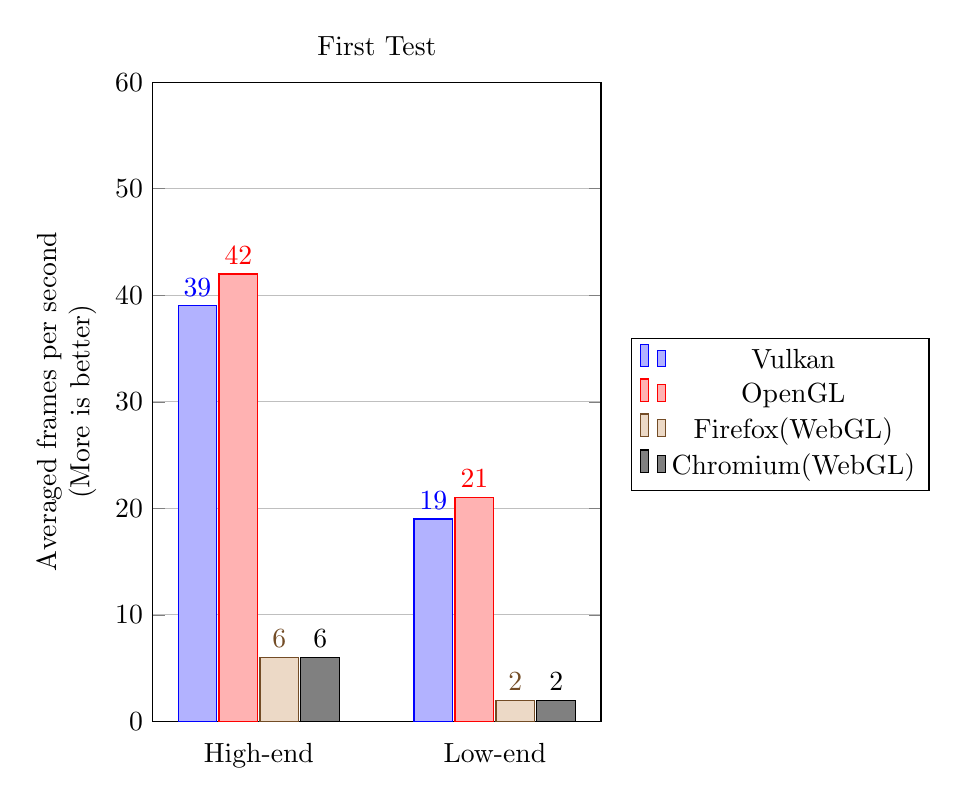
\begin{tikzpicture}
\begin{axis} [
    title = First Test,
    ylabel style={align=center}, ylabel=Averaged frames per second\\(More is better),
    nodes near coords,
    nodes near coords align={vertical},
    width = 0.6*\textwidth,
    height = 0.8*\textwidth,
    major x tick style = transparent,
    ybar=2*\pgflinewidth,
    bar width=14pt,
    ymajorgrids = true,
    symbolic x coords={High-end, Low-end},
    xtick = data,
    scaled y ticks = false,
    enlarge x limits=0.45,
    ymin=0,
    ymax=60,
    legend style={at={(1.4, 0.6)}, anchor=north},
]
\addplot coordinates {(High-end, 39) (Low-end, 19)}; %Vulkan
\addplot coordinates {(High-end, 42) (Low-end, 21)}; %OpenGL
\addplot coordinates {(High-end, 6) (Low-end, 2)}; %Firefox
\addplot coordinates {(High-end, 6) (Low-end, 2)}; %Chromium
\legend{Vulkan, OpenGL, Firefox(WebGL), Chromium(WebGL)}
\end{axis}
\end{tikzpicture}
\caption{Colored Cubes Test}
\label{fig:test1}
\end{figure}

\begin{figure}[!ht]
\center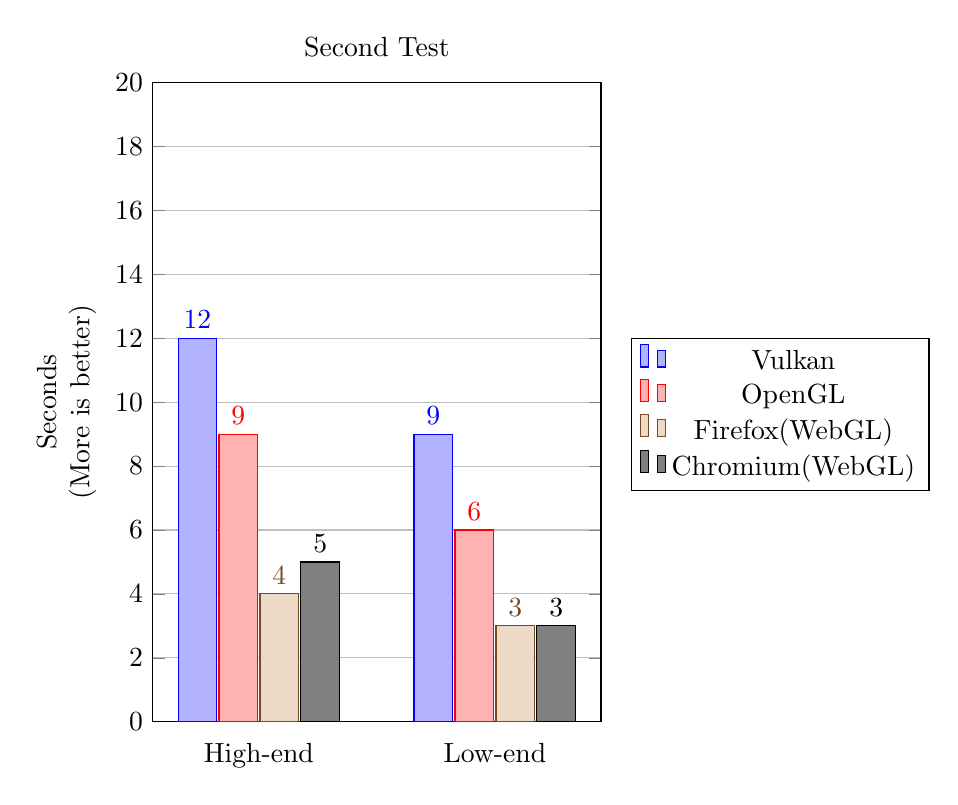
\begin{tikzpicture}
\begin{axis} [
    title = Second Test,
    ylabel style={align=center}, ylabel=Seconds\\(More is better),
    nodes near coords,
    nodes near coords align={vertical},
    width = 0.6*\textwidth,
    height = 0.8*\textwidth,
    major x tick style = transparent,
    ybar=2*\pgflinewidth,
    bar width=14pt,
    ymajorgrids = true,
    symbolic x coords={High-end, Low-end},
    xtick = data,
    scaled y ticks = false,
    enlarge x limits=0.45,
    ymin=0,
    ymax=20,
    legend style={at={(1.4, 0.6)}, anchor=north},
]
\addplot coordinates {(High-end, 12) (Low-end, 9)}; %Vulkan
\addplot coordinates {(High-end, 9) (Low-end, 6)}; %OpenGL
\addplot coordinates {(High-end, 4) (Low-end, 3)}; %Firefox
\addplot coordinates {(High-end, 5) (Low-end, 3)}; %Chromium
\legend{Vulkan, OpenGL, Firefox(WebGL), Chromium(WebGL)}
\end{axis}
\end{tikzpicture}
\caption{Colored Cone test}
\label{fig:test2}
\end{figure}



\end{document}
